\chapter{Nick's Lab}

Nestled near a fence behind Nick's home sits a small wood frame building. The
building is old enough that it must have been there before the nearby home was even 
built.  Inside of this building are several wooden workbenches filled with equipment
used to study electricity. The test gear is surrounded by a sea of wires. 

On the back wall of the building is a small window that opens up to the pasture
on the other side of the fence. Several Arabian horses spend their days in that
pasture, and occasionally wander up to see what is goin on inside of the
building. 

This is Nick's lab. When he is not studying for school, Nick spends a lot of
time in this lab playing with electricity and trying to figure out what it can do.
Nick keeps a supply of carrots handy when he works, and when a horse sticks its
head in the window, a carrot is usually delivered to keep him happy.

Nick has run electrcity to this building from his home so he can work on his experements.
Nick has always been fascinated by Eelectricity. When he was a kid, he took some wire, a
light buld and a battery and built a simple flashlight. That silly gadget was
used to read magazines under the covers in his room when he was supposed to be
sleeping.

Seated in Nick's lab is the last member of our gang of students. Leo is tearing
apart an old radio to see what makes it work. The radio dates back to the 1940s
and Leo's grandfather told him he used it to listen to the BBC during World War
II. The radio was sitting unused in an upstairs room in his grandfather's
house. Two wires were running from the back of the radio out a nearby window.
One of the wires extended up into a tree some distance from the house. The
other wire ran down the side of the house and was connected to a water pipe
that went into the ground. Leo had to disconnect those wires before he took the
radio to Nick's lab for proper study.

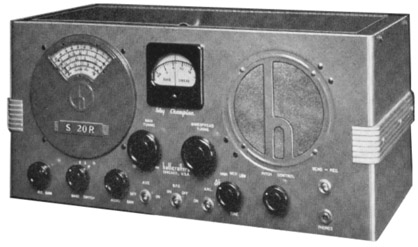
\includegraphics[width=0.6\textwidth]{hls020.jpg}

Leo is one of those strange people who loves to take things apart. Sometimes he
even manages to put them back together again. The back of the radio is made os
some kind of wood his grandfather called bakelite. Leo removed the five screws
holding the bakelite panel in place so he could see what was inside. Then he
plugged the radio into the wall socket and turned the knob on the front of the
radio. That knob was supposed to power up the radio and adjust the volume
according to his grandfather.

Leo was not quite sure what to expect, but looking inside he saw a set of seven
glass gadgets all of which were glowing and giving off quite a bit of heat. "This is
crazy" Leo muttered to himself!

There was nothing coming out of the radio. That might be because Leo had not
hooked up those two wires. Maybe those were needed to make it really work
properly.

The rest of the gang arrived as Leo was pondering the glow inside of his radio.
Alan piped up first.

"Hey Leo, I see you have managed to light up some old vacuum tubes! Those were
common when dinosaurs roamed the Earth."

"Funny, Alan. I just want to understand how this old thing manages to produce
sound."

"You really need to attach an antenna to that thing" was Nick's comment. 

Leo was still puzzled. "But how does a wire sitting up in the sky manage to
make the radio work?".

"Electromagnetic waves induce a current in the wire which the radio processes
into sound."

Ada chimes in. "Leave it to Alan to speak in tounges that mean nothing to the
rest of us! I guess we all have tome studying to do"

Nick has other ideas in mind.

"I thought we were here to see some real sparks fly."

"Fine, as long as we do not get burned by anything." Ada was just being a bit
cautious. All these folks knew they were immortal, at least until they reached
35 years old! Still, it never hurts to be careful, especially in Nick's lab!

Nick walks over to another workbench. Sitting in the middle of this bench is a
cardboad tube about a foot long with thin wire wound around it from top to
bottom. At the bottom of this tube is another coil of wire attached to some
electronic gadgets and finally attached to a power supply plugged into the
wall. At the top of the long tube is a silver donut made out of aluminum. 

"Leo, hit the lights!"

Nick flips the switch and sparks several inches lone shoot out of the donut,
dancing in the air. The smel of ozone fills the room.

"That is definitely way cooler than Alan's miswired switch!" says Ada.

Leo is intrigued. "It looks like electricity zooming through those wires
managed to generate something that made lightning fly away from that donut. Did
the coil make that happen?"

Alan contributes more of his vast wisdom. "When you make electricity move
around in circles like that, an electromagnetic wave is produced that moves
away from the coil. What is really cool is what happens if you hold a
flourescent light near this coil. It lights up with no connections. Somehow
that electromagnetic wave gets turned back inot enough electricity to light the
bulb."

Aha! That is the basis of radio!" Leo has figured out why the antenna wire is
needed to produce any sound. "But what is the other wire all about? The one
connected to the water pipe."
